\documentclass[11pt,a4paper]{article}
\parindent0pt
\parskip10pt
\raggedright
\usepackage{amsmath}
\usepackage{float}
\usepackage{graphicx}
\usepackage{listings}
\usepackage{caption}
\usepackage{subcaption}
\usepackage[T1]{fontenc}
\usepackage[brazilian]{babel}
\usepackage{geometry}
\usepackage{lmodern}
\usepackage[usenames,dvipsnames,svgnames,table]{xcolor}
\begin{document}

\newcommand*{\titleGP}[6]{\begingroup
\centering
\vspace*{\baselineskip}
\rule{\textwidth}{1.6pt}\vspace*{-\baselineskip}\vspace*{2pt}
\rule{\textwidth}{0.4pt}\\[\baselineskip]
{\Huge {#1}} % Title
\rule{\textwidth}{0.4pt}\vspace*{-\baselineskip}\vspace{3.2pt}
\rule{\textwidth}{1.6pt}\\[\baselineskip]
\scshape
{\Large {#2}\\[\baselineskip] % Description
{#3}} % location and date
\vspace*{2\baselineskip}
{\huge {#4}} % authors
\vspace*{2\baselineskip}
{#6} % middle thing (ex: img)
\vfill
{\Large {#5}} % footer
\endgroup}

\pagenumbering{gobble}
\newgeometry{left=20mm,right=20mm}
\titleGP{title}{asdasdasd}{february 2015}{author}{asdasd}{asdasd}
\restoregeometry
\pagenumbering{arabic}


\tableofcontents


\part{Part One}

%\chapter{Chapter One}

\section{Haskell}

\lstset{language=haskell}
\begin{lstlisting}[frame=single]
main = do
  as <- getArgs
  return as
\end{lstlisting}

\section{C}

\lstset{language=C}
\begin{lstlisting}[frame=none]
int main (args* char[]){
   return c + 3;
}
\end{lstlisting}

%\chapter{Chapter Two}

{\color{yellow}This text is yellow}
{\color{red}This is red!}
{\color{green}greeeeeeeeeeeeeeeeeen}

\begin{center}\centering{\tt asdasdasdasdasda
sdfasdfa
sdfasdfa
sdfasdfasdf
asdfasfdasdf hey hey}\end{center}

\begin{equation}
a^5 = b^5 + c^5 + \int^{\inf}_{0}dx^5
\end{equation}

\part{Part Two}

\section{Math giberish}

\subsection{Maths}

$$\vec{a}^5 + \mathbf{a} = \sin{3423414}$$

\begin{figure}[H]
\centering
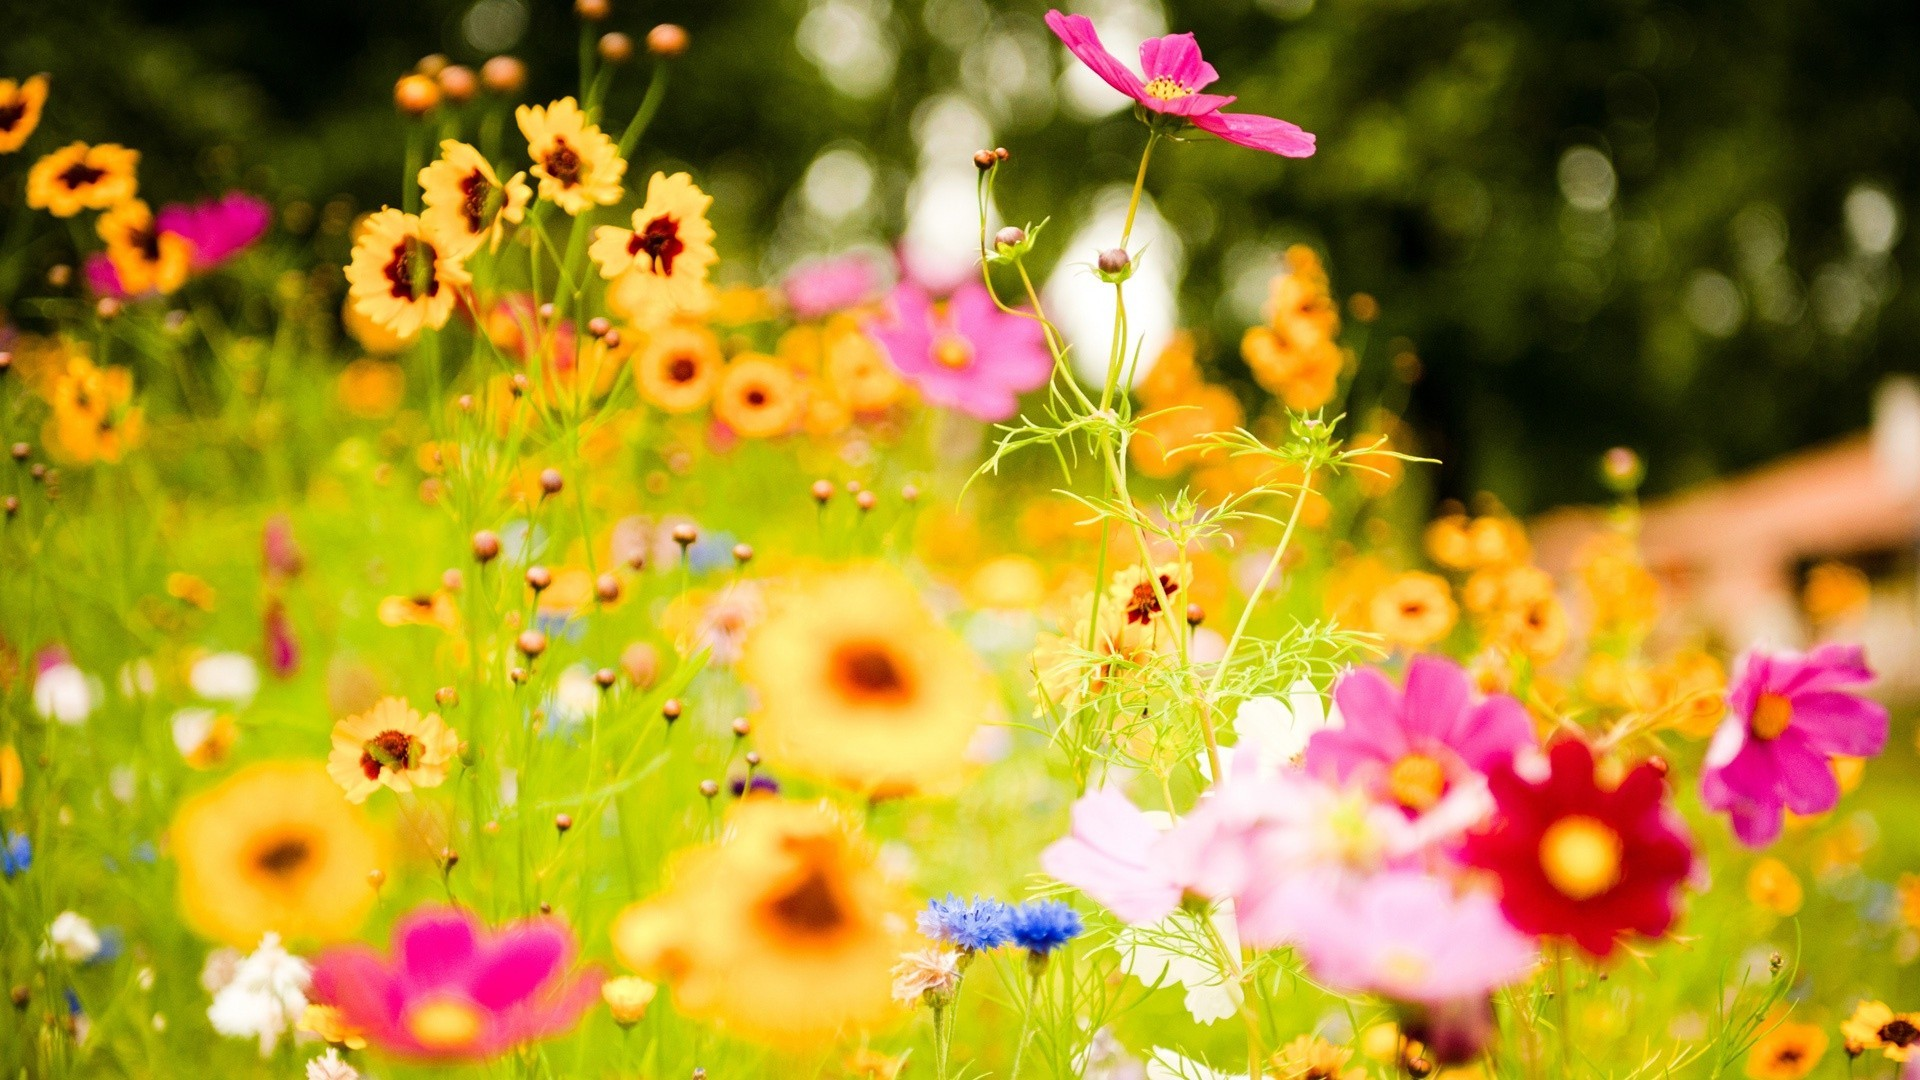
\includegraphics[width=10cm]{../../External/Images/flowers}
\caption{flowers}
\end{figure}

{\tt Richard Feynman}

{\tt asdasdasdasdasda
sdfasdfa
sdfasdfa
sdfasdfasdf
asdfasfdasdf hey hey}

\end{document}